\documentclass[11pt]{article}
\usepackage[margin=2.1cm]{geometry}
\usepackage{booktabs}
\usepackage{amsmath}
\usepackage{amssymb}
\usepackage{enumitem}
\usepackage{array}
\usepackage{listings}
\usepackage{xcolor}
\usepackage{tikz}
\usepackage[T1]{fontenc}
\usepackage{lmodern}

\setlength{\parindent}{0pt}
\setlength{\parskip}{3.6pt}
\newcommand{\code}[1]{\texttt{#1}}
\newcommand{\hr}{\vspace{2pt}\hrule\vspace{6pt}}
\renewcommand{\arraystretch}{1.12}

\definecolor{kw}{RGB}{0,90,160}
\definecolor{cmt}{RGB}{110,110,110}
\lstdefinestyle{vhdl}{
  language=VHDL, basicstyle=\ttfamily\footnotesize,
  keywordstyle=\color{kw}\bfseries, commentstyle=\color{cmt}\itshape,
  showstringspaces=false, columns=fullflexible, breaklines=true,
  frame=leftline, framesep=6pt, xleftmargin=8pt, aboveskip=6pt, belowskip=6pt
}
\lstset{style=vhdl}

\begin{document}

\begin{center}
{\Large\bfseries EE\,362 --- Pre-Lab 2: Solution}\\[2pt]
{\large Master--Slave Flip-Flop and the N-Bit Register}\\[4pt]
Fall 2026 \quad$\cdot$\quad 5 points \quad$\cdot$\quad TA marking guide
\end{center}
\hr

{\small Marking: Q1 = 2 points, Q2 = 1 point, Q3 = 2 points. Question 3 is the one
that predicts who will finish the lab. Mark it first.}

\vspace{4pt}\hr

\section*{Question 1 --- The timing diagram (2 points)}

\subsection*{The answer}

\begin{center}
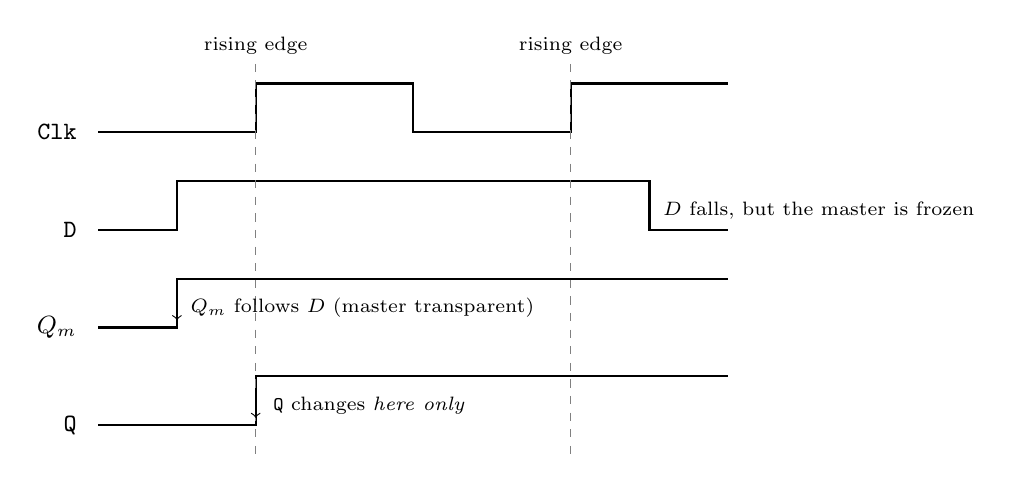
\begin{tikzpicture}[x=1.0cm, y=0.62cm]
  % time axis references
  \def\lo{0} \def\hi{1}
  % Clk: two full periods, starting low. low 0-2, high 2-4, low 4-6, high 6-8
  \node[left] at (-0.15, 0) {\small\code{Clk}};
  \draw[thick] (0,0) -- (2,0) -- (2,1) -- (4,1) -- (4,0) -- (6,0) -- (6,1) -- (8,1);
  % D: rises mid first low phase (t=1), falls mid second high phase (t=7)
  \node[left] at (-0.15,-2) {\small\code{D}};
  \draw[thick] (0,-2) -- (1,-2) -- (1,-1) -- (7,-1) -- (7,-2) -- (8,-2);
  % Qm: master transparent while Clk low. follows D during low phases; frozen while high
  \node[left] at (-0.15,-4) {\small$Q_m$};
  \draw[thick] (0,-4) -- (1,-4) -- (1,-3) -- (8,-3);
  % Q: slave copies master at rising edges only
  \node[left] at (-0.15,-6) {\small\code{Q}};
  \draw[thick] (0,-6) -- (2,-6) -- (2,-5) -- (8,-5);
  % edge markers
  \foreach \x in {2,6} \draw[dashed,gray] (\x,1.4) -- (\x,-6.6);
  \node[above] at (2,1.4) {\scriptsize rising edge};
  \node[above] at (6,1.4) {\scriptsize rising edge};
  \draw[->] (1,-3.3) -- (1,-3.85);
  \node[right,font=\scriptsize] at (1.05,-3.6) {$Q_m$ follows $D$ (master transparent)};
  \draw[->] (2,-5.3) -- (2,-5.85);
  \node[right,font=\scriptsize] at (2.1,-5.6) {\code{Q} changes \emph{here only}};
  \node[right,font=\scriptsize] at (7.05,-1.6) {$D$ falls, but the master is frozen};
\end{tikzpicture}
\end{center}

\textbf{What must be marked correct:}

\begin{enumerate}[leftmargin=2em,itemsep=2pt]
\item $Q_m$ changes \textbf{when \code{Clk} is low} and \code{D} changes --- the
master is transparent in the low phase.
\item \code{Q} changes \textbf{only at a rising edge}, never anywhere else.
\item When \code{D} falls during the \emph{high} phase (at the right of the
diagram), \textbf{neither $Q_m$ nor \code{Q} moves.} The master is closed, so the
new value cannot even get in. This is the point of the whole question.
\end{enumerate}

Accept any consistent clock phase, and accept a diagram where the student places
the $D$ transitions at slightly different times, provided the three facts above
hold.

\subsection*{The one sentence}

\begin{quote}
\textbf{Model answer:} \code{Q} changes only at the \textbf{rising edge} of the
clock. At every other instant the two latches are never open at the same time:
while the clock is low the master is open but the slave is closed, and while the
clock is high the slave is open but the master is closed. So there is never a path
from \code{D} straight through to \code{Q}.
\end{quote}

\textbf{Full credit} requires the idea \emph{never open at the same time}.
\textbf{Half credit:} ``because it is edge-triggered'' --- true but circular, and
it does not answer \emph{what prevents} it.

\vspace{4pt}\hr

\section*{Question 2 --- Interface and sensitivity list (1 point)}

\subsection*{The entity}

\begin{lstlisting}
entity RegN is
    generic (
        N : positive := 32
    );
    port (
        D   : in  std_logic_vector(N - 1 downto 0);
        Clk : in  std_logic;
        Ld  : in  std_logic;
        Rst : in  std_logic;
        Q   : out std_logic_vector(N - 1 downto 0)
    );
end entity RegN;
\end{lstlisting}

Required: the \code{generic} declared \emph{before} the \code{port}, the vector
ports sized \code{N - 1 downto 0}, and \code{Clk}, \code{Ld}, \code{Rst} as single
bits. \textbf{Control is narrow, data is wide.}

Do not accept \code{N downto 0} (that is $N+1$ bits) or a generic without a
default value --- the default is what lets \code{RegN} be instantiated without a
\code{generic map} later.

\subsection*{The sensitivity list --- and why it is not Lab 1's rule}

\begin{center}
\begin{tabular}{lcl}
\toprule
signal & in the list? & why \\
\midrule
\code{Clk} & \textbf{yes} & the process must wake to test for an edge \\
\code{Rst} & \textbf{yes} & \textbf{asynchronous}: it must act without waiting for an edge \\
\code{Ld}  & no & only read \emph{at} the edge, and the edge is a \code{Clk} event \\
\code{D}   & no & same reason: sampled at the edge, never between edges \\
\bottomrule
\end{tabular}
\end{center}

\begin{lstlisting}
process (Clk, Rst)
\end{lstlisting}

\begin{quote}
\textbf{Model answer:} A clocked process needs the clock and every asynchronous
control signal, and nothing else. \code{Ld} and \code{D} are read only at the
rising edge; the process is already awake at that instant because \code{Clk}
changed, so adding them changes nothing.
\end{quote}

\textbf{The contrast with Lab 1, worth saying out loud at check-off:}

\begin{center}
\begin{tabular}{lll}
\toprule
& Lab 1 (latch) & Lab 2 (register) \\
\midrule
rule & every signal the process \emph{reads} & the clock + asynchronous controls only \\
list & \code{(Clr, En, D)} & \code{(Clk, Rst)} \\
why & level-sensitive: \code{D} matters continuously & edge-triggered: \code{D} matters only at the edge \\
\bottomrule
\end{tabular}
\end{center}

\textbf{Common wrong answers:}
\begin{itemize}[leftmargin=1.6em,itemsep=1pt]
\item \code{(Clk, Rst, Ld, D)} --- \emph{half credit}. It simulates correctly and
synthesises correctly, so it is not a bug; but the student has applied Lab 1's
rule without noticing that the rule changed. Ask them when \code{D} is read.
\item \code{(Clk)} alone --- \emph{no credit}. The reset is then not asynchronous:
it would wait for a clock edge, which contradicts row 0 of the table.
\item Including \code{Q} --- \emph{no credit}. \code{Q} is written, not read.
\end{itemize}

\vspace{4pt}\hr

\section*{Question 3 --- The test plan (2 points)}

This is the same question as Section 5 of the report, and it is the one that
matters.

\subsection*{Model answer}

\begin{center}
\small
\begin{tabular}{c>{\raggedright\arraybackslash}p{6.0cm}>{\raggedright\arraybackslash}p{7.2cm}}
\toprule
\# & Stimulus, and \emph{when} & What it proves \\
\midrule
1 & Assert \code{Rst} \textbf{between} two edges, with \code{Ld}=1 and \code{D} all ones
  & The reset is \textbf{asynchronous}. If it only acts at an edge, this fails. \\
2 & After a falling edge set \code{D} to a known pattern, \code{Ld}=1, then wait for the rising edge
  & The register \textbf{loads} at the edge (row 3). \\
3 & \textbf{Between} two rising edges, toggle \code{D} three times
  & \textbf{The edge vector.} \code{Q} must not move at all. A transparent latch fails here. \\
4 & Let the next rising edge arrive after those toggles
  & The edge captures the \textbf{last} value before it, not an earlier one. \\
5 & Set \code{Ld}=0, change \code{D}, allow a rising edge
  & Row 2: an edge with \code{Ld} low \textbf{holds}. \\
6 & Load a pattern that is neither all-zeros nor all-ones (e.g.\ \code{x"DEADBEEF"})
  & Bit ordering is right; a swapped or stuck bit is visible. \\
\bottomrule
\end{tabular}
\end{center}

Accept a different order, and accept extra vectors. \textbf{Vectors 1, 3 and 5
must be present} in some form. Vector 3 is worth the most.

\subsection*{The closing question: which vector would a latch fail?}

\begin{quote}
\textbf{Model answer:} A transparent latch would \textbf{fail vector 3}. While the
enable is high a latch follows \code{D} continuously, so toggling \code{D} between
edges would move \code{Q}. It would pass vectors 1, 2, 5 and 6, because those only
check values sampled around an edge, and a latch that happens to be open at that
moment produces the same answer.
\end{quote}

\textbf{Mark strictly here.} If a student names any vector other than the
toggle-between-edges vector, they have not yet understood the difference between
level-sensitive and edge-triggered, and they will struggle in the build. Sixty
seconds at the bench now is worth twenty minutes later.

\subsection*{Why vector 3 alone is not sufficient}

Worth saying to strong students: vector 3 proves \code{Q} does not follow \code{D}
between edges. It does \emph{not} prove the register ever loads. A design with
\code{Q} permanently stuck at its reset value also passes vector 3. That is why
vectors 2 and 3 must appear together --- \textbf{one proves it moves, the other
proves it does not move too often.}

\vspace{6pt}
\hr
{\small \textbf{If a student got Q3 wrong but Q1 right}, they can usually repair
the test plan in two minutes by reading their own timing diagram: the vector that
matters is the interval where \code{D} moves and \code{Q} does not.}

\end{document}
